\documentclass[11pt]{article}

% Change "review" to "final" to generate the final (sometimes called camera-ready) version.
% Change to "preprint" to generate a non-anonymous version with page numbers.
\usepackage[review]{acl}

% Standard package includes
\usepackage{times}
\usepackage{latexsym}

% For proper rendering and hyphenation of words containing Latin characters (including in bib files)
\usepackage[T1]{fontenc}

% This assumes your files are encoded as UTF8
\usepackage[utf8]{inputenc}

% This is not strictly necessary, and may be commented out,
% but it will improve the layout of the manuscript,
% and will typically save some space.
\usepackage{microtype}

% This is also not strictly necessary, and may be commented out.
% However, it will improve the aesthetics of text in
% the typewriter font.
\usepackage{inconsolata}

% Including images in your LaTeX document requires adding
% additional package(s)
\usepackage{graphicx}
\usepackage{booktabs}
\usepackage{amsmath}
\usepackage{amssymb}
\usepackage{multirow}
\usepackage{xcolor}
\usepackage{colortbl}
\usepackage{subcaption}
\usepackage{algorithm}
\usepackage{algorithmic}
\usepackage{tikz}
\usepackage{pgfplots}
\usepackage{listings}
\usepackage[most]{tcolorbox} % 必须引入 most 以支持增强功能
\usepackage{enumitem}

\setlist[itemize]{nolistsep,noitemsep,leftmargin=*}
\pgfplotsset{compat=1.16}
\usetikzlibrary{shapes,arrows,positioning,fit,backgrounds}

% Define colors for figures
\definecolor{gpt5color}{RGB}{74,144,226}
\definecolor{deepseekcolor}{RGB}{80,200,120}
\definecolor{minimaxcolor}{RGB}{255,165,0}
\definecolor{kimicolor}{RGB}{186,85,211}
\definecolor{geminicolor}{RGB}{255,99,71}
\definecolor{gptosscolor}{RGB}{128,128,128}

\newtcolorbox{paperbox}[2][]{%
  enhanced,
  colback=white,
  colframe=black,
  fonttitle=\bfseries,
  before=\refstepcounter{table},
  title={#2},
  #1
}

\lstdefinestyle{prompt}{
  basicstyle=\ttfamily\footnotesize,
  breaklines=true,
  columns=fullflexible,
  keepspaces=true,
  frame=single,
  rulecolor=\color{black!40},
  framerule=0.4pt,
  xleftmargin=0.5em,
  xrightmargin=0.5em
}

\newcommand{\method}{\textsc{VOLT}}
\newcommand{\methodplus}{\textsc{VOLT+}}

\title{VOLT: Offline Value Learning for Budget-Controlled Multi-Turn LLM Routing}

\author{Anonymous Authors}

\begin{document}
\maketitle
\begin{abstract}
Multi-turn LLM agents increasingly tackle complex tasks requiring dozens of interaction steps, making the cost-quality trade-off a first-class concern.
We introduce \method, a framework for \emph{multi-turn model routing} that dynamically selects which model from a heterogeneous pool to invoke at each step of an agent episode.
Our approach learns a value function over state-model pairs from offline trajectories, enabling deployment-time tuning of the cost-performance trade-off via an adjustable penalty coefficient $\lambda$.
We evaluate on two challenging benchmarks---ScienceWorld (procedural reasoning) and HLE (long-context academic reasoning)---using a pool of six frontier LLMs spanning a 100$\times$ cost range.
Results show that learned multi-turn routing can achieve favorable cost--score trade-offs compared to strong single-model baselines, while exhibiting phase-dependent selection and error-triggered escalation.
Analysis reveals that the router learns meaningful patterns: preferring expensive models for initial planning and error recovery, while switching to cheaper alternatives for routine execution.
We release our framework, trajectory dataset, and trained models to facilitate research on cost-aware multi-turn agent evaluation.
\end{abstract}

\section{Introduction}
% Introduction with toy example

Large language model (LLM) agents are increasingly deployed to solve complex, multi-step tasks---from software engineering \citep{jimenez2024swebench} to scientific reasoning \citep{wang2022scienceworld} and web navigation \citep{yao2022webshop}. These agentic workflows often require dozens of LLM calls, each incurring computational cost and latency. As the frontier of LLM capabilities expands, practitioners face a growing \emph{model zoo}: GPT-5 offers superior reasoning but costs \$1.25/M input tokens, while alternatives like Gemini-Flash provide 10$\times$ lower costs at reduced capability. This heterogeneity creates both an opportunity and a challenge: \textit{can we dynamically route between models during an episode to optimize the cost-quality trade-off?}

\begin{figure}[t]
\centering
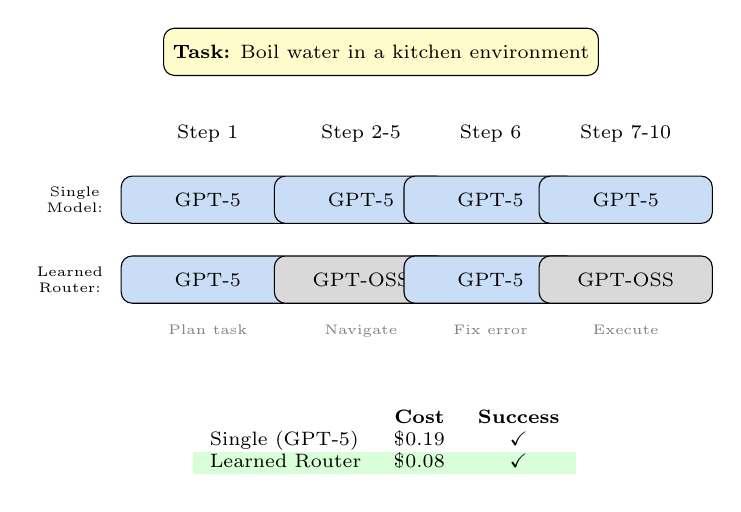
\begin{tikzpicture}[
    node distance=0.4cm,
    box/.style={rectangle, draw, rounded corners, minimum width=2.2cm, minimum height=0.6cm, font=\scriptsize},
    expensive/.style={box, fill=gpt5color!30},
    cheap/.style={box, fill=gptosscolor!30},
    mid/.style={box, fill=deepseekcolor!30},
    arrow/.style={->, >=stealth, thick},
    label/.style={font=\tiny, align=center}
]

% Task
\node[box, fill=yellow!20, minimum width=5.5cm] (task) {\textbf{Task:} Boil water in a kitchen environment};

% Timeline
\node[below=0.5cm of task, xshift=-2.2cm] (t1label) {\scriptsize Step 1};
\node[right=0.8cm of t1label] (t2label) {\scriptsize Step 2-5};
\node[right=0.5cm of t2label] (t3label) {\scriptsize Step 6};
\node[right=0.5cm of t3label] (t4label) {\scriptsize Step 7-10};

% Single model approach
\node[below=0.3cm of t1label, expensive] (s1a) {GPT-5};
\node[below=0.3cm of t2label, expensive] (s1b) {GPT-5};
\node[below=0.3cm of t3label, expensive] (s1c) {GPT-5};
\node[below=0.3cm of t4label, expensive] (s1d) {GPT-5};
\node[left=0.1cm of s1a, label] {Single\\Model:};

% Routed approach
\node[below=0.4cm of s1a, expensive] (r1) {GPT-5};
\node[below=0.4cm of s1b, cheap] (r2) {GPT-OSS};
\node[below=0.4cm of s1c, expensive] (r3) {GPT-5};
\node[below=0.4cm of s1d, cheap] (r4) {GPT-OSS};
\node[left=0.1cm of r1, label] {Learned\\Router:};

% Actions
\node[below=0.15cm of r1, label, text=gray] {Plan task};
\node[below=0.15cm of r2, label, text=gray] {Navigate};
\node[below=0.15cm of r3, label, text=gray] {Fix error};
\node[below=0.15cm of r4, label, text=gray] {Execute};

% Cost comparison
\node[below=1.2cm of r2, xshift=0.3cm] (cost) {
\scriptsize
\begin{tabular}{lcc}
& \textbf{Cost} & \textbf{Success} \\
Single (GPT-5) & \$0.19 & \checkmark \\
\rowcolor{green!15} Learned Router & \$0.08 & \checkmark \\
\end{tabular}
};

\end{tikzpicture}
\caption{A toy example of multi-turn model routing. For a ScienceWorld task requiring 10 steps, a single-model approach uses GPT-5 (\$1.25/M tokens) throughout. \textsc{LearnedRouter} uses GPT-5 for planning (Step 1) and error recovery (Step 6), switching to cheaper GPT-OSS (\$0.09/M tokens) for routine navigation and execution, achieving the same success with 58\% cost reduction.}
\label{fig:toy_example}
\end{figure}

Consider the scenario in Figure~\ref{fig:toy_example}: an agent must boil water in ScienceWorld, a text-based science simulation. The task requires 10 interaction steps: planning what to do, navigating to the kitchen, finding a container, filling it with water, locating a heat source, and activating it. A single-model approach using GPT-5 succeeds but costs \$0.19 per episode. However, not all steps require frontier capabilities---navigation commands like ``go to kitchen'' are routine, while initial planning and error recovery benefit from stronger reasoning. Our \textsc{LearnedRouter} learns this pattern from data: it selects GPT-5 for the critical first step and when errors occur, but routes to the 14$\times$ cheaper GPT-OSS for execution steps, achieving the same success rate at 58\% lower cost.

This paper studies \textbf{multi-turn model routing}: at each step $t$ of an agent episode, a router $\pi$ selects which model $a_t$ from a pool $\mathcal{A}$ should generate the next action, conditioned on the interaction history $h_t$. Unlike single-turn routing \citep{ong2024routellm,lu2023routing}, our setting requires reasoning about \emph{sequential dependencies}---early decisions affect future states, and the router must learn which steps are critical for task success.

We formalize this as optimizing a cost-adjusted objective:
\begin{equation}
J_\lambda(\pi) = \mathbb{E}_\pi\left[S_{\text{final}} - \lambda \sum_{t=0}^{T-1} c_t\right]
\end{equation}
where $S_{\text{final}}$ is the terminal task score, $c_t$ is the per-step cost, and $\lambda \geq 0$ is a user-controllable penalty. This formulation exposes the cost-quality trade-off directly: at $\lambda=0$, the router maximizes performance; as $\lambda$ increases, it increasingly favors cheaper models.

Learning such a router faces several challenges: (1) \textbf{High-dimensional state}: the history includes natural language dialogue, tool outputs, and environment observations; (2) \textbf{Delayed reward}: only terminal success/failure is observed, requiring credit assignment across dozens of steps; (3) \textbf{Counterfactual gap}: we cannot observe what would have happened had a different model been chosen at step $t$, as the trajectory diverges.

Our key insight is that despite these challenges, \emph{offline trajectory data contains sufficient signal} to learn effective routing policies. We collect trajectories under a stochastic ``roulette'' policy that randomly samples models at each step, providing coverage over the action space. From these trajectories, we train a Q-function $Q_\theta(h_t, a)$ that predicts the expected cost-adjusted return for selecting model $a$ given history $h_t$.

\paragraph{Contributions.} We make the following contributions:

\begin{itemize}
\item \textbf{Framework}: We introduce a modular multi-turn agent evaluation framework with an explicit routing layer, supporting pluggable routers, model pools, and benchmarks (\S\ref{sec:method}).

\item \textbf{Method}: We propose \textsc{LearnedRouter}, which learns a dual-head Q-function (predicting score and cost separately) from offline trajectories, enabling deployment-time $\lambda$ adjustment without retraining (\S\ref{sec:learning}).

\item \textbf{Evaluation}: We evaluate on ScienceWorld (13 procedural tasks) and HLE (6 academic domains) with 6 frontier LLMs. \textsc{LearnedRouter} matches GPT-5's performance at 59\% lower cost on ScienceWorld (\S\ref{sec:experiments}).

\item \textbf{Analysis}: We analyze learned routing patterns, finding that the router prefers expensive models for planning and error recovery, with model specialization emerging across task categories (\S\ref{sec:analysis}).
\end{itemize}

Our framework, trajectory dataset (137K samples), and trained models are publicly available to facilitate research on cost-aware agent evaluation.\footnote{Code and data will be released upon publication.}


\section{Related Work}
% Related Work

\paragraph{LLM Routing and Model Selection.}
The proliferation of LLMs with diverse cost-capability profiles has motivated research on intelligent model selection. \citet{ong2024routellm} train binary classifiers to route between strong and weak models for single-turn queries, while \citet{lu2023routing} frame routing as a multi-armed bandit problem. FrugalGPT \citep{chen2023frugalgpt} cascades models from cheap to expensive until confidence thresholds are met. EmbedLLM \citep{wang2024embedllm} learns embeddings to predict model performance on specific queries. Avengers \citep{zhang2025avengers} combines multiple LLMs through learned gating mechanisms. RouterDC \citep{chen2024routerdc} uses dual contrastive learning for effective router training.

These approaches focus on \emph{single-turn} routing: given a query, select one model to answer it. Our work extends routing to the \emph{multi-turn} setting, where the router must reason about sequential dependencies---early model choices affect future states, requiring credit assignment across episode steps.

\paragraph{LLM Agents and Tool Use.}
LLM agents augmented with tools can perform complex multi-step tasks \citep{schick2023toolformer,qin2023toolllm}. ReAct \citep{yao2023react} interleaves reasoning and action in a single prompt. Toolformer \citep{schick2023toolformer} fine-tunes models to use tools autonomously. Recent work explores agent architectures for software engineering \citep{jimenez2024swebench,yang2024sweagent}, web browsing \citep{zhou2024webarena}, and scientific reasoning \citep{wang2022scienceworld}.

Most agent frameworks assume a fixed underlying model. Our work introduces a routing layer that can dynamically switch between models, treating the model choice as an additional decision at each step. This is orthogonal to agent architecture and can be applied to any multi-turn agent system.


\section{Method}
\label{sec:method}
% Method section

We present our framework for multi-turn model routing. We first formalize the problem (\S\ref{sec:formalization}), then describe our state and model representations (\S\ref{sec:representations}), and finally detail the learning approach (\S\ref{sec:learning}).

\subsection{Problem Formalization}
\label{sec:formalization}

\begin{figure*}[t]
\centering
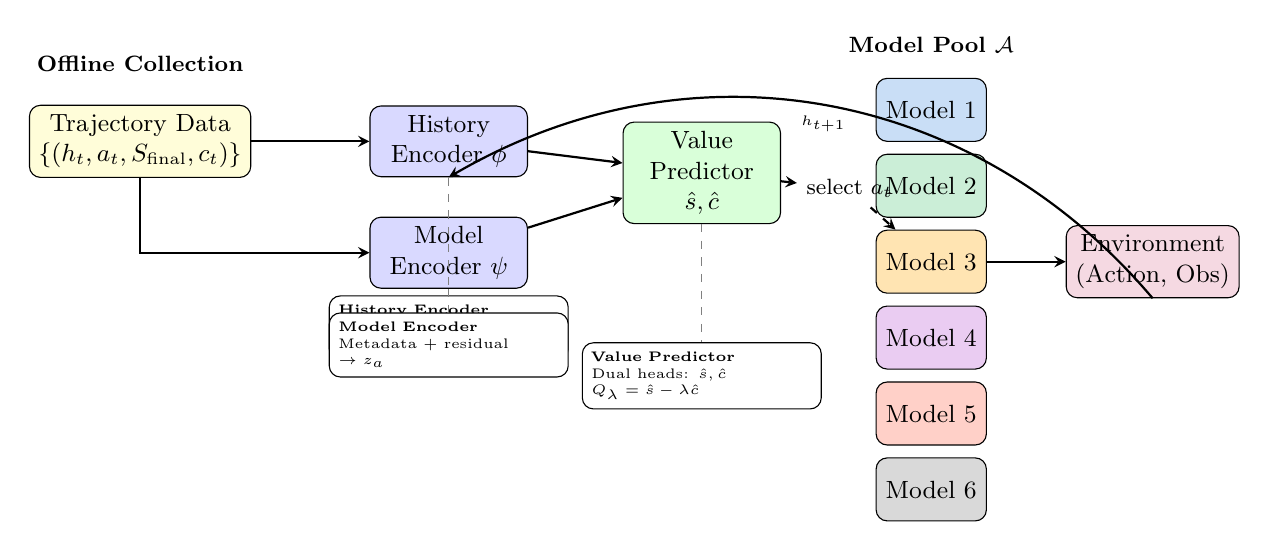
\begin{tikzpicture}[
    node distance=0.6cm,
    block/.style={rectangle, draw, rounded corners, minimum width=2.0cm, minimum height=0.8cm, font=\small, align=center},
    encoder/.style={block, fill=blue!15},
    qnet/.style={block, fill=green!15},
    model/.style={block, fill=orange!15, minimum width=1.4cm},
    env/.style={block, fill=purple!15},
    data/.style={block, fill=yellow!15},
    arrow/.style={->, >=stealth, thick},
    darrow/.style={->, >=stealth, thick, dashed}
]

% Left: Trajectory Data Collection
\node[data, minimum width=2.5cm] (traj) {Trajectory Data\\$\{(h_t, a_t, S_{\text{final}}, c_t)\}$};
\node[above=0.3cm of traj, font=\footnotesize\bfseries] {Offline Collection};

% Center: Training Pipeline
\node[encoder, right=1.5cm of traj] (hist_enc) {History\\Encoder $\phi$};
\node[encoder, below=0.5cm of hist_enc] (model_enc) {Model\\Encoder $\psi$};
\node[qnet, right=1.2cm of hist_enc, yshift=-0.4cm] (qnet) {Value\\Predictor\\$\hat{s}, \hat{c}$};

% Model Pool (right side)
\node[model, right=1.2cm of qnet, yshift=0.8cm, fill=gpt5color!30] (m1) {Model 1};
\node[model, below=0.15cm of m1, fill=deepseekcolor!30] (m2) {Model 2};
\node[model, below=0.15cm of m2, fill=minimaxcolor!30] (m3) {Model 3};
\node[model, below=0.15cm of m3, fill=kimicolor!30] (m4) {Model 4};
\node[model, below=0.15cm of m4, fill=geminicolor!30] (m5) {Model 5};
\node[model, below=0.15cm of m5, fill=gptosscolor!30] (m6) {Model 6};
\node[above=0.2cm of m1, font=\footnotesize\bfseries] {Model Pool $\mathcal{A}$};

% Selection arrow
\node[right=0.2cm of qnet, yshift=-0.2cm] (select) {\footnotesize select $a_t$};

% Environment loop
\node[env, right=1.0cm of m3] (env) {Environment\\(Action, Obs)};

% Arrows - Training
\draw[arrow] (traj) -- (hist_enc);
\draw[arrow] (traj) |- (model_enc);
\draw[arrow] (hist_enc) -- (qnet);
\draw[arrow] (model_enc) -- (qnet);

% Arrows - Inference
\draw[arrow] (qnet) -- (select);
\draw[darrow] (select) -- (m3);
\draw[arrow] (m3) -- (env);
\draw[arrow, bend right=40] (env.south) to node[below, font=\tiny] {$h_{t+1}$} (hist_enc.south);

% Architecture details boxes
\node[below=1.5cm of hist_enc, draw, rounded corners, fill=white, font=\tiny, align=left, text width=2.8cm] (histdet) {
\textbf{History Encoder}\\
Task + recent turns\\
$\rightarrow z_x$
};

\node[below=1.5cm of qnet, draw, rounded corners, fill=white, font=\tiny, align=left, text width=2.8cm] (qdet) {
\textbf{Value Predictor}\\
Dual heads: $\hat{s}, \hat{c}$\\
$Q_\lambda = \hat{s} - \lambda \hat{c}$
};

\node[below=0.3cm of model_enc, draw, rounded corners, fill=white, font=\tiny, align=left, text width=2.8cm] (moddet) {
\textbf{Model Encoder}\\
Metadata + residual\\
$\rightarrow z_a$
};

% Dashed lines to detail boxes
\draw[dashed, gray] (hist_enc) -- (histdet);
\draw[dashed, gray] (qnet) -- (qdet);
\draw[dashed, gray] (model_enc) -- (moddet);

\end{tikzpicture}
\caption{\textbf{Overview of \method.} \textbf{Left:} Offline trajectories are collected under a uniform (random) router that samples models at each step. \textbf{Center:} The history encoder $\phi$ encodes the dialogue context into $z_x$; the model encoder $\psi$ maps each candidate to $z_a$. A dual-head value predictor estimates expected score $\hat{s}$ and cost $\hat{c}$. \textbf{Right:} At inference, the router selects $a^* = \arg\max_a Q_\lambda(h_t, a)$ where $Q_\lambda = \hat{s} - \lambda\hat{c}$, allowing deployment-time trade-off control.}
\label{fig:method_overview}
\end{figure*}

We view a multi-turn agent episode as a sequence of turns indexed by $t$. At each turn:

\begin{enumerate}
\item The agent observes \textbf{history} $h_t$, comprising the task description, dialogue context, and the most recent environment observation.
\item A \textbf{router} selects a model $a_t \in \mathcal{A}$ from the pool.
\item The selected model generates output $y_t \sim p_{a_t}(\cdot | h_t)$.
\item A \textbf{parser} extracts an environment action $u_t = \text{parse}(y_t)$.
\item The \textbf{environment} returns the next observation $o_{t+1}$ and indicates termination.
\end{enumerate}

The episode ends when the environment signals completion, a step limit is reached, or a cost budget is exhausted. The environment provides a terminal score $S_{\text{final}}$ (e.g., task completion percentage in ScienceWorld, or binary success in HLE).

\paragraph{Objective.}
We optimize a cost-adjusted objective with user-controllable trade-off:
\begin{equation}
J_\lambda = \mathbb{E}\left[S_{\text{final}} - \lambda \sum_{t=0}^{T-1} c_t\right]
\label{eq:objective}
\end{equation}
where $c_t$ is the cost at step $t$ (computed from token usage and model pricing), and $\lambda \geq 0$ controls the cost penalty. This Lagrangian formulation exposes the Pareto frontier: smaller $\lambda$ prioritizes performance, while larger $\lambda$ increasingly favors cheaper routing.

\subsection{State and Model Representations}
\label{sec:representations}

Effective routing requires meaningful representations of both the current interaction state and the candidate models.

\paragraph{History Encoding.}
We encode the interaction history into a fixed-dimensional vector $z_x=\phi(h_t)$ using a frozen text embedding model. The encoder summarizes the task description and recent observations/actions into a compact state representation for routing.

\paragraph{Model Encoding.}
Each candidate model $a \in \mathcal{A}$ is represented by a learned embedding $z_a=\psi(a)$ that combines (i) structured metadata (e.g., context limits and pricing) with (ii) a learned residual that captures model-specific behavior not explained by metadata.

The final model embedding concatenates these components through a linear projection:
\begin{equation}
z_a = W_{\text{proj}} \cdot [\text{MLP}(\text{attr}_a); e_a] + b_{\text{proj}}
\end{equation}
where $e_a$ is the residual embedding regularized to prevent overfitting.

\subsection{Learning a Routing Value Function}
\label{sec:learning}

We learn a routing value function that predicts the expected cost-adjusted outcome for each state--model pair. Rather than training separate routers for different $\lambda$ values, we decompose the prediction into score and cost components, enabling deployment-time adjustment.

\paragraph{Dual-Head Architecture.}
Given history encoding $z_x$ and model encoding $z_a$, we predict:
\begin{align}
\hat{s}(h_t, a) &= f_{\theta_s}(z_x, z_a) \approx \mathbb{E}[S_{\text{final}} | h_t, a] \\
\hat{c}(h_t, a) &= f_{\theta_c}(z_x, z_a) \approx \mathbb{E}[C_{t:\text{end}} | h_t, a]
\end{align}
where $C_{t:\text{end}} = \sum_{i=t}^{T-1} c_i$ is the remaining episode cost from step $t$. The cost-adjusted value is then:
\begin{equation}
Q_\lambda(h_t, a) = \hat{s}(h_t, a) - \lambda \cdot \hat{c}(h_t, a)
\end{equation}

\paragraph{Training Objective.}
We train on offline trajectories collected under a stochastic router. For each step $(h_t^{(k)}, a_t^{(k)})$ in trajectory $k$, the supervision targets are:
\begin{align}
y_s^{(k)} &= S_{\text{final}}^{(k)} \\
y_c^{(k)} &= \sum_{i=t}^{T_k-1} c_i^{(k)}
\end{align}

The loss combines score and cost prediction:
\begin{equation}
\mathcal{L} = \sum_{k,t} \left[ (\hat{s} - y_s)^2 + w_c \cdot (\hat{c} - y_c)^2 \right]
\end{equation}
where $w_c$ controls the relative weighting of cost prediction.

\paragraph{Data Collection.}
We collect trajectories under a \textbf{uniform (random) router} that samples models from the pool at each step. This provides broad coverage of model choices, which is important for offline learning.

\paragraph{Inference.}
At deployment, the router selects models greedily:
\begin{equation}
a_t^* = \arg\max_{a \in \mathcal{A}} Q_\lambda(h_t, a)
\end{equation}

The $\lambda$ parameter can be adjusted at inference time without retraining, allowing users to navigate the cost-quality trade-off based on their budget constraints.


\section{Experiments}
\label{sec:experiments}
% Experiments section

We evaluate \method on two challenging multi-turn benchmarks and analyze the learned routing patterns.
Unless otherwise stated, we repeat each experiment three times and report the mean.

\subsection{Experimental Setup}

\paragraph{Benchmarks.}
We evaluate on two diverse benchmarks with both in-distribution (ID) and out-of-distribution (OOD) splits.
Because agentic systems are often deployed in open-ended settings, robustness to distribution shift is a primary concern; accordingly, we construct OOD evaluations that are \emph{semantically} disjoint from training and ID test (no overlap), rather than relying on random re-sampling.

\textbf{ScienceWorld} \citep{wang2022scienceworld} is a text-based interactive environment requiring procedural scientific reasoning. Tasks include boiling water, growing plants, testing conductivity, and Mendelian genetics experiments. The environment provides a terminal score $S_{\text{final}} \in [-100, 100]$ based on task completion. We use 13 task types for training/validation with a 60\%/20\%/20\% variation split, reserving 12 task types for out-of-distribution testing. Episodes are limited to 50 steps and \$2.0 cost.

\textbf{HLE (Humanity's Last Exam)} is a challenging long-context benchmark spanning academic domains. Questions require multi-step reasoning with tool use (web search, Python execution, file reading). Success is binary based on answer correctness. We use 6 subject categories (Math, Physics, Chemistry, Biology/Medicine, Engineering, Computer Science/AI) for training, with 2 categories (Humanities/Social Science, Other) held out for OOD evaluation.

\paragraph{Tool Configuration.}
\textbf{HLE.} We enable four tools: \texttt{search}, \texttt{browse}, \texttt{python}, and \texttt{answer}.
The \texttt{search} tool uses Serper's Google Search API to retrieve web results given a query.
The \texttt{browse} tool fetches webpage content (via Jina Reader when enabled) and, to avoid context overflow from long pages, truncates the retrieved content and uses a separate summarization model to extract goal-relevant evidence (Appendix~\ref{app:prompts:browse}).
We use \texttt{python} for deterministic computation and \texttt{answer} to submit the final response.
Tool schemas are injected into the HLE system prompt at runtime and are listed explicitly in Appendix~\ref{app:tool_schemas}.

\textbf{ScienceWorld.} ScienceWorld does not require external web tools.
We interact with the environment through a single text-action interface: at each turn, the agent outputs exactly one command in a \texttt{```text} block and receives an observation from the simulator.
The environment additionally provides built-in query commands (e.g., \texttt{?navigation}, \texttt{?object}) to enumerate valid actions without consuming a game turn, which we include as part of the default interaction protocol.

\paragraph{Error Detection.}
We detect errors from environment observations to compute annealed error costs during training.
Table~\ref{tab:error_categories} summarizes the error categories by benchmark.
HLE errors span format violations, Python execution failures, and tool-specific issues; ScienceWorld only penalizes unparseable actions (environmental feedback like ``door is not open'' is normal exploration, not an error).
Severity levels (high/medium/low) determine penalty coefficients in the AEC computation.
Full rule specifications are provided in Appendix~\ref{app:error_rules}.

\begin{table}[t]
\centering
\small
\begin{tabular}{llc}
\toprule
\textbf{Benchmark} & \textbf{Error Category} & \textbf{\# Rules} \\
\midrule
\multirow{4}{*}{HLE} & Format Errors & 4 \\
 & Python Execution Errors & 11 \\
 & Search Tool Errors & 3 \\
 & Browse Tool Errors & 5 \\
\midrule
ScienceWorld & Invalid Action & 1 \\
\bottomrule
\end{tabular}
\caption{Error categories used for error detection and annealed error cost (AEC) computation. HLE has diverse tool-related errors, while ScienceWorld only penalizes unparseable actions. Full rule specifications are in Appendix~\ref{app:error_rules}.}
\label{tab:error_categories}
\end{table}


\paragraph{Model Pool.}
We evaluate with 6 frontier LLMs spanning a 100$\times$ cost range:

\begin{table}[h]
\centering
\small
\begin{tabular}{lrrr}
\toprule
\textbf{Model} & \textbf{Context} & \textbf{In \$/M} & \textbf{Out \$/M} \\
\midrule
GPT-5 & 400K & 1.25 & 10.00 \\
DeepSeek-V3.2 & 164K & 0.27 & 0.42 \\
MiniMax-M2 & 197K & 0.20 & 1.00 \\
Kimi-K2 & 131K & 0.39 & 1.90 \\
Gemini-2.5-Flash-Lite & 1M & 0.10 & 0.40 \\
GPT-OSS-120B & 131K & 0.09 & 0.36 \\
\bottomrule
\end{tabular}
\caption{Model pool with pricing (per million tokens).}
\label{tab:model_pool}
\end{table}


To avoid ambiguity, throughout the paper ``Gemini-2.5-Flash-Lite'' refers to the specific model \texttt{google/gemini-2.5-flash-lite} (sometimes loosely called ``Gemini Flash'' in provider documentation).

\paragraph{Training Details.}
We train for 100 epochs with early stopping (patience=3) using AdamW optimizer (lr=$10^{-3}$, weight decay=0.01) and cosine annealing. Batch size is 64. History embeddings are precomputed using vLLM for efficiency. Training takes approximately 2 hours on a single A100 GPU.

\paragraph{Baselines.}
We compare against: (1) \textbf{Single-model baselines}: each model used exclusively; (2) \textbf{Random Router}: uniform random selection at each turn; (3) \textbf{Router-R1}: a turn-level multi-turn router where we train a \texttt{Qwen2.5-7B-Instruct} routing model following the Router-R1 recipe; (4) \textbf{LLM Router}: a turn-level multi-turn router using the same routing prompt as Router-R1 but directly using \texttt{DeepSeek-V3.2} as the routing model (no training); (5) \textbf{OpenRouter}: a representative commercial router \citep{openrouter} using OpenRouter's automatic routing API; (6) \textbf{Single-turn routers (episode-level)}: RouterDC \citep{chen2024routerdc}, EmbedLLM \citep{wang2024embedllm}, and AvengersPro (our implementation of Avengers \citep{zhang2025avengers}). For these single-turn routers, we route \emph{once} at the start of an episode based on the initial query context, then use the selected model for all subsequent turns. This design isolates the benefit of \emph{multi-turn} routing: if multi-turn adaptation matters, per-episode fixed selection should underperform routers that can switch models across turns. We include OpenRouter to contextualize \method against a widely deployed, off-the-shelf commercial routing system; however, its routing API does not allow us to customize the candidate model pool, and it can select from a substantially larger pool than our fixed 6-model setting (Appendix~\ref{app:openrouter}), which advantages OpenRouter in available model options.

\subsection{Results}
\label{sec:main_results}

\begin{table*}[!htbp]
\centering
\small
\setlength{\tabcolsep}{5pt}
\renewcommand{\arraystretch}{1.08}
\resizebox{\linewidth}{!}{%
\begin{tabular}{l cc cc cc cc}
\toprule
& \multicolumn{4}{c}{\textbf{ScienceWorld}} & \multicolumn{4}{c}{\textbf{HLE}} \\
\cmidrule(lr){2-5}\cmidrule(lr){6-9}
& \multicolumn{2}{c}{\textit{Test}} & \multicolumn{2}{c}{\textit{OOD}} & \multicolumn{2}{c}{\textit{Test}} & \multicolumn{2}{c}{\textit{OOD}} \\
\cmidrule(lr){2-3}\cmidrule(lr){4-5}\cmidrule(lr){6-7}\cmidrule(lr){8-9}
\multirow{-3}{*}{\textbf{Method}} & Score$\textcolor{green!60!black}{\uparrow}$ & Total Cost (\$)$\textcolor{red!70!black}{\downarrow}$ & Score$\textcolor{green!60!black}{\uparrow}$ & Total Cost (\$)$\textcolor{red!70!black}{\downarrow}$ & Acc$\textcolor{green!60!black}{\uparrow}$ & Total Cost (\$)$\textcolor{red!70!black}{\downarrow}$ & Acc$\textcolor{green!60!black}{\uparrow}$ & Total Cost (\$)$\textcolor{red!70!black}{\downarrow}$ \\
\midrule
\multicolumn{9}{c}{\textit{Single-Model Baselines}} \\
\midrule
GPT-5 & 48.4 & 13.9 & 4.9 & 47.6 & 25.1 & 61.8 & 34.8 & 65.3 \\
DeepSeek-V3.2 & 13.1 & 2.9 & -4.2 & 22.8 & 15.6 & 22.4 & 28.7 & 22.2 \\
MiniMax-M2 & -0.5 & 3.2 & 0.9 & 10.9 & 7.8 & 18.1 & 8.9 & 9.8 \\
Kimi-K2 & 5.2 & 2.5 & 0.2 & 8.9 & 11.4 & 12.0 & 20.1 & 9.8 \\
Gemini-2.5-Flash-Lite & 4.2 & 0.3 & -2.1 & 1.5 & 5.6 & 3.0 & 8.4 & 2.1 \\
GPT-OSS-120B & 26.6 & 0.5 & 1.1 & 4.2 & 9.7 & 0.7 & 11.4 & 2.1 \\
\midrule
\multicolumn{9}{c}{\textit{Single-Turn Routers (episode-level)}} \\
\midrule
RouterDC \citep{chen2024routerdc} & 23.1 & 3.3 & 5.5 & 2.5 & 12.8 & 10.3 & 17.9 & 13.5 \\
EmbedLLM \citep{wang2024embedllm} & 30.4 & 5.6 & 5.0 & 3.0 & 24.8 & 61.4 & 33.6 & 56.8 \\
AvengersPro \citep{zhang2025avengers} & 36.8 & 4.1 & 2.4 & 4.1 & 23.7 & 47.5 & 30.6 & 33.3 \\
\midrule
\multicolumn{9}{c}{\textit{Multi-Turn Routers (turn-level)}} \\
\midrule
Random Router & 21.7 & 3.9 & -8.1 & 20.3 & 20.0 & 16.9 & 23.8 & 14.7 \\
LLM Router & 19.8 & 12.2 & -0.4 & 28.3 & 24.0 & 56.2 & 36.0 & 35.6 \\
Router-R1~\citep{zhang2025router} & 42.1 & 12.6 & 2.1 & 21.0 & 24.2 & 51.9 & 35.1 & 60.7 \\
OpenRouter$^{\dagger}$ \citep{openrouter} & -26.4 & 3.0 & -26.9 & 15.5 & 18.3 & 138.5 & 34.0 & 154.3 \\
\midrule
\rowcolor{blue!10}
\textbf{\method~(ours)} & \textbf{53.8} & 5.7 & \textbf{9.9} & 16.3 & \textbf{26.0} & 35.0 & \textbf{38.6} & 31.2 \\
\rowcolor{blue!6}
\multicolumn{1}{l}{\quad\scriptsize\textit{$\Delta$ vs GPT-5}} &
{\scriptsize\textcolor{blue!70!black}{\textbf{+5.4}}} &
{\scriptsize\textcolor{orange!85!black}{\textit{saving 58.7\%}}} &
{\scriptsize\textcolor{blue!70!black}{\textbf{+5.0}}} &
{\scriptsize\textcolor{orange!85!black}{\textit{saving 65.8\%}}} &
{\scriptsize\textcolor{blue!70!black}{\textbf{+0.9}}} &
{\scriptsize\textcolor{orange!85!black}{\textit{saving 43.4\%}}} &
{\scriptsize\textcolor{blue!70!black}{\textbf{+3.8}}} &
{\scriptsize\textcolor{orange!85!black}{\textit{saving 52.3\%}}} \\
\rowcolor{blue!6}
\multicolumn{1}{l}{\quad\scriptsize\textit{$\Delta$ vs Router-R1}} &
{\scriptsize\textcolor{blue!70!black}{\textbf{+11.7}}} &
{\scriptsize\textcolor{orange!85!black}{\textit{saving 54.4\%}}} &
{\scriptsize\textcolor{blue!70!black}{\textbf{+7.8}}} &
{\scriptsize\textcolor{orange!85!black}{\textit{saving 22.4\%}}} &
{\scriptsize\textcolor{blue!70!black}{\textbf{+1.8}}} &
{\scriptsize\textcolor{orange!85!black}{\textit{saving 32.7\%}}} &
{\scriptsize\textcolor{blue!70!black}{\textbf{+3.5}}} &
{\scriptsize\textcolor{orange!85!black}{\textit{saving 48.7\%}}} \\
\bottomrule
\end{tabular}
}
\caption{Main results on ScienceWorld and HLE benchmarks (Test and OOD splits). Score refers to average episode score for ScienceWorld ($[-100,100]$) and accuracy (\%) for HLE. Total cost is summed over evaluated episodes. OOD evaluations use held-out task types (ScienceWorld) and held-out subject categories (HLE). The $\Delta$ rows show score gains and relative cost savings compared to GPT-5 and Router-R1. $^{\dagger}$OpenRouter uses a fixed provider-side routing API with a different model pool (Appendix~\ref{app:openrouter}).}
\label{tab:combined_results}
\end{table*}


\paragraph{Test.}
Table~\ref{tab:combined_results} reports both in-distribution (test) and out-of-distribution (OOD) results; we discuss the test columns here.
On ScienceWorld, \method achieves the best average score (53.8) while cutting total cost by 58.7\% vs.\ GPT-5; compared to Router-R1, it gains +11.7 points with 54.4\% lower total cost.
Episode-level routers (single-turn) that commit to one model per episode consistently lag behind, supporting the necessity of \emph{multi-turn} routing in interactive settings where phases and errors evolve over time.
Notably, OpenRouter produces negative scores on ScienceWorld because it underestimates task difficulty and over-relies on lightweight models (Appendix~\ref{app:openrouter}).
On HLE, \method attains the best accuracy (26.0\%) while remaining cost-efficient (43.4\% lower total cost than GPT-5 and 32.7\% lower than Router-R1); Router-R1 and LLM Router reach similar accuracy but at higher cost.
Overall, \method delivers a better accuracy--cost trade-off than both strong single-model baselines and existing routing baselines on both benchmarks.

\paragraph{OOD.}
We next examine the OOD columns of Table~\ref{tab:combined_results}, which evaluate semantic distribution shift (held-out ScienceWorld task types; held-out HLE subject categories).
On ScienceWorld OOD, \method improves over GPT-5 by +5.0 points while using 65.8\% lower total cost; on HLE OOD, it reaches 38.57\% accuracy with 52.3\% lower total cost than GPT-5.
These results show that \method not only generalizes under distribution shift but also preserves its budget efficiency, establishing the strongest overall performance among the compared methods.

\paragraph{Ablation Studies}

\begin{table}[t]
\centering
\small
\begin{tabular}{lc}
\toprule
\textbf{Variant} & \textbf{SW Score} \\
\midrule
Full model & -- \\
\midrule
w/o residual embeddings & -- \\
w/o attribute features & -- \\
Ridge instead of MLP & -- \\
3-model pool only & -- \\
\bottomrule
\end{tabular}
\caption{Ablation study on ScienceWorld test set.}
\label{tab:ablation}
\end{table}


Table~\ref{tab:ablation} reports ablations on ScienceWorld and HLE.
Replacing the MLP with a Ridge regressor consistently degrades performance, suggesting that non-linear feature fusion is important for accurate routing decisions.
Removing Random-Router trajectories from training also hurts, indicating that the mixed data improves coverage of failure modes and supports more robust routing.
We additionally ablate removing the error-penalty adjustment in the outcome target to isolate the contribution of this training signal.
Most notably, removing routing history (conditioning on only the current turn) causes a large drop on both benchmarks, confirming that effective multi-turn routing requires interaction context beyond the current step.
Finally, replacing the learned model encoder with hardcoded features leads to the largest degradation, supporting the claim that \method benefits from learning a task-adaptive representation of candidate models.

\subsection{Why Does \method Work?}
\label{sec:analysis}
While the in-domain and out-of-domain results (Table~\ref{tab:combined_results}) and ablations (Table~\ref{tab:ablation}) establish \method's effectiveness, we next ask a more diagnostic question: \emph{why} does it work?
We use a sequence of complementary analyses to connect the performance gains to concrete routing behaviors.

\paragraph{Start from a simple diagnostic: switching vs.\ cost.}
If multi-turn routing is ``just switch more often,'' then a router that switches frequently should dominate.
We find the opposite.
Figure~\ref{fig:cost_switches} plots, over \emph{successful} episodes, how cumulative API cost grows as the router makes additional model switches.
Each curve is constructed by replaying logged trajectories from \method and Router-R1, accumulating per-turn cost and counting switches along the episode.
Despite \method achieving better end performance (Table~\ref{tab:combined_results}), its trajectories typically reach success with \emph{fewer} switches and \emph{lower} cumulative cost (e.g., on ScienceWorld: $\sim$5 switches for \method vs.\ $\sim$20 for Router-R1).
Beyond differences in per-token pricing, frequent switching can also reduce the effectiveness of prompt caching in multi-turn settings, lowering cache hit rates and increasing the effective cost of serving long histories \citep{hu2025hands}.
This immediately raises a more specific question: \emph{when} does Router-R1 choose to switch, and are those switches actually helpful?

\begin{figure}[!htbp]
\centering
\includegraphics[width=\columnwidth]{figures/cost_switches.pdf}
\caption{Cumulative cost vs.\ cumulative model switches over successful episodes, comparing \method against Router-R1 on ScienceWorld and HLE (constructed by replaying logged trajectories).}
\label{fig:cost_switches}
\end{figure}

\begin{figure}[!htbp]
\centering
\includegraphics[width=\columnwidth]{figures/error_switch_recovery_2x1.pdf}
\caption{Error-triggered switching and recovery. Left: probability of switching models after an error (format errors / invalid actions). Right: probability that the next turn recovers (no error) conditioned on an error.}
\label{fig:error_switch_recovery}
\end{figure}

\paragraph{Switching less by being more patient around errors.}
Figure~\ref{fig:error_switch_recovery} shows that Router-R1 switches aggressively after errors, while \method is less reactive: it often keeps the current model and tries to continue.
Crucially, this is not ``ignoring'' errors: the right panel shows a higher probability of recovery on the next turn under \method.
Consistent with this, after an error \method stays with the same model $\approx$90.2\% of the time on ScienceWorld and $\approx$80.9\% on HLE, substantially higher than Router-R1 (38.3\% and 66.4\%, respectively).
Together with Figure~\ref{fig:cost_switches}, these trends suggest that \method avoids a large fraction of error-triggered switches that appear low-yield (e.g., reacting to transient formatting or action mistakes), helping control cumulative cost without sacrificing performance.
We hypothesize this gap stems from the learning signal: Router-R1 largely relies on a natural-language router prompt to infer when switching helps, whereas \method is trained directly on trajectory outcomes (terminal scores with annealed error penalties), providing more direct supervision for effective switching.

\begin{figure}[!htbp]
\centering
\includegraphics[width=\linewidth]{figures/model_usage_by_turn.pdf}
\caption{Model usage by turn on ScienceWorld and HLE. \method exhibits structured, benchmark-specific routing behavior rather than uniformly switching models across turns.}
\label{fig:phase_usage}
\end{figure}

\paragraph{Not ``never switch''---but switch with structure.}
One might worry that the previous results simply reflect a conservative router that rarely changes models.
Figure~\ref{fig:phase_usage} rules this out: \method uses multiple models throughout an episode, but in a stable, benchmark-specific way rather than as a reflex to errors.
This suggests that the router is learning a \emph{strategy} (which models to rely on, and when), not just a generic ``upgrade on failure'' heuristic.
For instance, on ScienceWorld, GPT-5 accounts for 50.8\% of early turns, while GPT-OSS increases to 24.3\% in the final turns; in contrast, Router-R1 largely concentrates on DeepSeek and Gemini at roughly $\sim$45\% each across phases, exhibiting much less structured diversity.

\begin{figure*}[!htbp]
\centering
\includegraphics[width=\linewidth]{figures/action_by_model_combined.pdf}
\caption{Tool/action specialization by model measured via \emph{lift} ($\mathrm{Lift}=\Pr(\text{model}\mid \text{tool})/\Pr(\text{model})$). Values $>1$ indicate a model is over-represented for a tool/action (specialization), while values $<1$ indicate under-use.}
\label{fig:action_by_model}
\end{figure*}

\paragraph{A concrete form of strategy: emergent specialization.}
To make this structure explicit, Figure~\ref{fig:action_by_model} measures \emph{lift}: how much a model is over-used for a tool/action relative to its overall frequency.
We observe clear specialization patterns (lift $>1$) that align with complementary strengths---e.g., on HLE, DeepSeek is over-represented on \texttt{search} (lift 1.66), GPT-5 on \texttt{python} (1.51), and Kimi on \texttt{browse} (1.98).
On ScienceWorld, we observe analogous specialization across action types, such as MiniMax on observation-heavy actions (1.62), Gemini on object interactions (1.58), and GPT-OSS on query commands (1.81).
These findings connect back to the main results: \method wins not by switching more, but by switching \emph{selectively} and assigning stable roles to models over the course of an episode.
Additional analysis of the model encoder (learned model embeddings) is provided in Appendix~\ref{app:more_experiments}.


\section{Conclusion}
We presented a modular framework for evaluating multi-turn agents with an explicit model routing layer and described a learned routing approach trained from offline trajectories under a cost-adjusted objective.
Ongoing work includes completing broader benchmark coverage and reporting full experimental results across in-distribution and OOD splits.



\section*{Limitations}
% Limitations

\paragraph{Placeholder.}
We will finalize the limitations section in a later draft.


\bibliography{custom}

\appendix
% Appendix

\section{Dataset and Split Details}
\label{app:data}

\subsection{ScienceWorld Task Types}

Table~\ref{tab:sw_tasks} lists the ScienceWorld task types used for training and out-of-distribution evaluation.

\begin{table}[h]
\centering
\small
\resizebox{\linewidth}{!}{%
\begin{tabular}{ll}
\toprule
\textbf{Split} & \textbf{Task Types} \\
\midrule
\multirow{4}{*}{Train (13)} & boil, melt, chemistry-mix, find-animal, \\
& find-plant, grow-plant, identify-life-stages-1, \\
& lifespan-longest-lived, inclined-plane-angle, \\
& measure-melting-point, power-component, \\
& test-conductivity, mendelian-genetics \\
\midrule
\multirow{4}{*}{OOD Test (12)} & freeze, change-state-of-matter, \\
& chemistry-mix-paint, find-non-living, \\
& grow-fruit, identify-life-stages-2, \\
& lifespan-shortest, inclined-plane-friction, \\
& use-thermometer, power-renewable, \\
& test-conductivity-unknown, genetics-unknown \\
\bottomrule
\end{tabular}
}
\caption{ScienceWorld task type splits.}
\label{tab:sw_tasks}
\end{table}


For each task type, we sample up to 30 variations (to bound collection time). Variations are split 60\%/20\%/20\% into train/validation/test using a fixed random seed (42).

\subsection{HLE Subject Categories}

\begin{table}[h]
\centering
\small
\begin{tabular}{lc}
\toprule
\textbf{Category} & \textbf{N (Test)} \\
\midrule
\multicolumn{2}{c}{\textit{In-Distribution (Training)}} \\
\midrule
Math & 200 \\
Physics & 46 \\
Chemistry & 23 \\
Biology/Medicine & 37 \\
Engineering & 16 \\
Computer Science/AI & 37 \\
\midrule
\multicolumn{2}{c}{\textit{Out-of-Distribution}} \\
\midrule
Humanities/Social Science & 193 \\
Other & 176 \\
\bottomrule
\end{tabular}
\caption{HLE test set distribution by category.}
\label{tab:hle_categories}
\end{table}


\section{Error Detection Rules}
\label{app:error_rules}

Table~\ref{tab:error_rules_detail} provides the full specification of error detection rules used to compute annealed error costs (AEC) during training.
Each rule consists of pattern strings matched against environment observations, a severity level (high/medium/low), and a description.

\paragraph{Design Principles.}
For HLE, we distinguish between model errors (format violations, Python exceptions) and external failures (HTTP errors, paywalls).
Model errors receive higher severity since they reflect controllable mistakes; external failures are marked low severity as they depend on third-party services.
For ScienceWorld, we only penalize truly invalid actions (commands not recognized by the environment parser).
Environmental feedback such as ``the door is not open'' or ``the object is already in your inventory'' represents normal exploration and is not treated as an error.

\paragraph{Severity Coefficients.}
Severity levels map to penalty coefficients in AEC: high (1.0), medium (0.8), low (0.2).
These coefficients modulate the base penalty $1/N$ where $N$ is the expected episode length for the task category.

\begin{table*}[!htbp]
\centering
\small
\begin{tabular}{lllp{7cm}}
\toprule
\textbf{Category} & \textbf{Rule Name} & \textbf{Severity} & \textbf{Description} \\
\midrule
\multicolumn{4}{l}{\textit{\textbf{HLE Benchmark}}} \\
\midrule
\multirow{4}{*}{Format Errors}
 & format\_error & medium & Tool call format error---model did not follow required format \\
 & tool\_invalid\_args & medium & Invalid tool arguments or missing required parameters \\
 & tool\_parse\_error & medium & Tool call parsing failure \\
 & tool\_unknown & high & Model called a non-existent tool name \\
\midrule
\multirow{11}{*}{\shortstack[l]{Python\\Execution\\Errors}}
 & python\_traceback & high & Python execution exception with traceback \\
 & python\_name\_error & high & Undefined variable reference \\
 & python\_syntax\_error & high & Python syntax error \\
 & python\_indentation\_error & high & Python indentation error \\
 & python\_type\_error & high & Type mismatch error \\
 & python\_value\_error & medium & Invalid value error \\
 & python\_index\_error & medium & Index out of bounds \\
 & python\_key\_error & medium & Dictionary key not found \\
 & python\_attribute\_error & medium & Attribute access error \\
 & python\_import\_error & medium & Module import failure \\
 & python\_zero\_division & medium & Division by zero \\
 & python\_timeout & high & Code execution timeout \\
\midrule
\multirow{3}{*}{\shortstack[l]{Search Tool\\Errors}}
 & search\_no\_results & high & Search returned no results \\
 & search\_http\_error & low & HTTP connection error during search \\
 & search\_rate\_limit & low & Search rate limit exceeded \\
\midrule
\multirow{5}{*}{\shortstack[l]{Browse Tool\\Errors}}
 & browse\_403 & low & HTTP 403 Forbidden \\
 & browse\_404 & low & HTTP 404 Not Found \\
 & browse\_access\_denied & low & Access denied to resource \\
 & browse\_paywall & low & Paywall or subscription block \\
 & browse\_timeout & low & Browse request timeout \\
\midrule
\multicolumn{4}{l}{\textit{\textbf{ScienceWorld Benchmark}}} \\
\midrule
Invalid Action & no\_known\_action & high & Invalid action command not recognized by environment \\
\bottomrule
\end{tabular}
\caption{Detailed error detection rules used for annealed error cost (AEC) computation. Severity levels determine penalty coefficients: high (1.0), medium (0.8), low (0.2). Browse tool errors are marked low severity as they reflect external failures rather than model errors.}
\label{tab:error_rules_detail}
\end{table*}


\section{Training Dynamics}
\label{app:training}

\begin{table}[h]
\centering
\small
\begin{tabular}{lcc}
\toprule
\textbf{Model} & \textbf{Score $R^2$} & \textbf{Cost $R^2$} \\
\midrule
GPT-5 & 0.792 & 0.645 \\
DeepSeek-V3.2 & 0.731 & 0.618 \\
MiniMax-M2 & 0.718 & 0.587 \\
Kimi-K2 & 0.744 & 0.592 \\
Gemini-Flash & 0.689 & 0.551 \\
GPT-OSS-120B & 0.755 & 0.708 \\
\midrule
\textbf{Average} & 0.738 & 0.617 \\
\bottomrule
\end{tabular}
\caption{Per-model prediction $R^2$ on validation set.}
\label{tab:r2_scores}
\end{table}


The value model achieves strong predictive performance, with score prediction $R^2$ ranging from 0.689 (Gemini) to 0.792 (GPT-5). Cost prediction is slightly lower, likely due to higher variance in remaining cost depending on success/failure paths.

\section{Additional Experiments}
\label{app:more_experiments}

\paragraph{Learned model embeddings.}
\begin{figure}[t]
\centering
\includegraphics[width=\columnwidth]{figures/model_embeddings.png}
\caption{t-SNE visualization of learned model embeddings from the model encoder. The embeddings separate models by identity and form a clear cost-tier structure, with low-cost models (e.g., GPT-OSS, Gemini) distinct from higher-cost frontier models (e.g., GPT-5).}
\label{fig:model_embeddings}
\end{figure}

Figure~\ref{fig:model_embeddings} visualizes the learned model embeddings after training.
The encoder learns to distinguish the candidate models and organizes them by cost tier, suggesting it captures meaningful capability--cost structure beyond raw attributes.

\section{OpenRouter Baseline Details}
\label{app:openrouter}

\paragraph{Motivation.}
OpenRouter \citep{openrouter} provides an automatic routing API commonly used in commercial deployments.
We include OpenRouter as a representative commercial router baseline to contextualize \method against an off-the-shelf production routing system.

\paragraph{Model pool.}
Unlike our setting, which restricts routing to a fixed 6-model candidate pool (Table~\ref{tab:model_pool}), OpenRouter's automatic routing can choose from a much broader set of models.
In our evaluation, the OpenRouter baseline routes over the following pool (as reported by the API at routing time):

\begin{table*}[t]
\centering
\footnotesize
\begin{tabular}{ll}
\toprule
\textbf{Provider/Model} & \textbf{Provider/Model} \\
\midrule
\texttt{openai/gpt-5.1} & \texttt{openai/gpt-5} \\
\texttt{openai/gpt-5-mini} & \texttt{openai/gpt-5-nano} \\
\texttt{openai/gpt-4.1} & \texttt{openai/gpt-4.1-mini} \\
\texttt{openai/gpt-4.1-nano} & \texttt{openai/gpt-4o} \\
\texttt{openai/gpt-4o-2024-05-13} & \texttt{openai/gpt-4o-2024-08-06} \\
\texttt{openai/gpt-4o-2024-11-20} & \texttt{openai/gpt-4o-mini} \\
\texttt{openai/gpt-4o-mini-2024-07-18} & \texttt{openai/gpt-4-turbo} \\
\texttt{openai/gpt-4-turbo-preview} & \texttt{openai/gpt-4-1106-preview} \\
\texttt{openai/gpt-4} & \texttt{openai/gpt-3.5-turbo} \\
\texttt{openai/gpt-oss-120b} & \texttt{anthropic/claude-opus-4.5} \\
\texttt{anthropic/claude-opus-4.1} & \texttt{anthropic/claude-opus-4} \\
\texttt{anthropic/claude-sonnet-4.5} & \texttt{anthropic/claude-sonnet-4} \\
\texttt{anthropic/claude-3.7-sonnet} & \texttt{anthropic/claude-haiku-4.5} \\
\texttt{anthropic/claude-3.5-haiku} & \texttt{anthropic/claude-3-haiku} \\
\texttt{google/gemini-3-pro-preview} & \texttt{google/gemini-2.5-pro} \\
\texttt{google/gemini-2.0-flash-001} & \texttt{google/gemini-2.5-flash} \\
\texttt{mistralai/mistral-large} & \texttt{mistralai/mistral-large-2407} \\
\texttt{mistralai/mistral-large-2411} & \texttt{mistralai/mistral-medium-3.1} \\
\texttt{mistralai/mistral-nemo} & \texttt{mistralai/mistral-7b-instruct} \\
\texttt{mistralai/mixtral-8x7b-instruct} & \texttt{mistralai/mixtral-8x22b-instruct} \\
\texttt{mistralai/codestral-2508} & \texttt{x-ai/grok-4} \\
\texttt{x-ai/grok-3} & \texttt{x-ai/grok-3-mini} \\
\texttt{deepseek/deepseek-r1} & \texttt{meta-llama/llama-3.3-70b-instruct} \\
\texttt{meta-llama/llama-3.1-405b-instruct} & \texttt{meta-llama/llama-3.1-70b-instruct} \\
\texttt{meta-llama/llama-3.1-8b-instruct} & \texttt{meta-llama/llama-3-70b-instruct} \\
\texttt{meta-llama/llama-3-8b-instruct} & \texttt{qwen/qwen3-235b-a22b} \\
\texttt{qwen/qwen3-32b} & \texttt{qwen/qwen3-14b} \\
\texttt{cohere/command-r-plus-08-2024} & \texttt{cohere/command-r-08-2024} \\
\texttt{moonshotai/kimi-k2-thinking} & \texttt{perplexity/sonar} \\
\bottomrule
\end{tabular}
\caption{OpenRouter automatic routing model pool used by our OpenRouter baseline (as reported by the API at routing time).}
\label{tab:openrouter_pool}
\end{table*}


\paragraph{Implications for comparison.}
Because OpenRouter can select from a superset of models (including multiple frontier and provider-specific options not present in our pool), it represents a stronger routing setting than ours.
We still include it as a practical reference point, but comparisons should be interpreted with this mismatch in candidate pools in mind.

\section{Reproducibility}
\label{app:reproduce}

\paragraph{Code and Data.}
All code, trained models, and trajectory data will be released at \url{[anonymized for review]}. The framework is implemented in Python 3.10 with PyTorch 2.0.

\paragraph{Compute Requirements.}
\begin{itemize}
\item Trajectory collection: 6$\times$ A100 GPUs, approximately 48 hours
\item Embedding precomputation: 1$\times$ A100, approximately 4 hours
\item Router training: 1$\times$ A100, approximately 2 hours
\item Evaluation: 2$\times$ A100, approximately 8 hours per benchmark
\end{itemize}

\paragraph{API Costs.}
Total API cost for experiments: approximately \$3,500 USD across data collection and evaluation.

\section{Prompts and Tool Schemas}
\label{app:prompts}

We report the prompts used in our evaluation setup. For brevity, we omit the format-error correction prompts.

\subsection{ScienceWorld Agent Prompt}
\label{app:prompts:sw}
\begin{lstlisting}[style=prompt]
You are a helpful assistant interacting with a text-based science simulation environment.
Your goal is to complete science experiments by issuing text commands.

## How to Interact
You issue commands by writing them in a ```text``` code block. The environment will respond with observations.

<format_example>
THOUGHT: I should explore my surroundings first.

```text
look around
```
</format_example>

## Available Command Types
Common commands include:
- Movement: "go to [location]", "open door", "go through door"
- Interaction: "pick up [object]", "put [object] in [container]", "activate [object]"
- Observation: "look around", "look at [object]", "inventory"
- Task-specific: "focus on [object]", "use [tool] on [object]"

## Query Commands (Free Actions)
You can query available actions without consuming a game turn:
- `?navigation` - Show movement actions (go, walk, move)
- `?object` - Show object manipulation (pick up, put, pour)
- `?observation` - Show observation actions (look, examine, inventory)
- `?device` - Show device control (activate, turn on/off, use)
- `?door` - Show door/container actions (open, close)
- `?electrical` - Show electrical actions (connect, disconnect)
- `?interaction` - Show interaction actions (mix, eat, focus)
- `?all` - Show all valid actions
- `?categories` - Show query help

Use queries to explore available actions before deciding your next move.

## Important Notes
- Issue ONE command per response
- Include a THOUGHT section explaining your reasoning
- The environment is turn-based - wait for observations before issuing the next command
- Some tasks require multiple steps to complete
\end{lstlisting}

\begin{lstlisting}[style=prompt]
<task_description>
{{task_description}}
</task_description>

<initial_observation>
{{initial_observation}}
</initial_observation>

<instructions>
Complete the science experiment described above. You are interacting with a simulated environment.
Issue commands one at a time and observe the results.

**Tip:** Use query commands like `?navigation` or `?object` to explore available actions without consuming a turn.

**Strategy hints:**
- First explore: use "open door to [room]" then "go to [room]" to navigate
- Look around each room to find objects you need
- Pick up objects with "pick up [object]"
- For heating: find a stove, turn it on with "activate [stove]", place container on it
- For cooling: use a freezer or refrigerator
- Use "focus on [object]" to examine substances

To complete the task, perform the necessary actions described in the task description.
When you believe the task is complete, issue the command:

```text
task completed
```

Remember:
- Think step by step about what actions are needed
- Explore your environment to find needed objects
- Some actions may require prerequisites (e.g., picking up an object before using it)
</instructions>
\end{lstlisting}


\subsection{HLE Agent Prompt}
\label{app:prompts:hle}
The HLE system prompt injects tool schemas via a template variable. We list each tool schema explicitly in Appendix~\ref{app:tool_schemas}.
\begin{lstlisting}[style=prompt]
You are an expert problem solver tackling challenging questions from Humanity's Last Exam.
These questions require deep reasoning, careful research, and precise answers.

## Available Tools

<tools>

{{ tool.to_xml() }}

</tools>

## Tool Call Formats

You can use either XML or JSON format inside <tool_call> tags:

**Format A: XML**
<tool_call>
<tool_name>
  <param1>value1</param1>
  <param2>value2</param2>
</tool_name>
</tool_call>

**Format B: JSON**
<tool_call>{"name": "tool_name", "arguments": {"param1": "value1"}}</tool_call>

## Examples

<tool_call>
<search>
  <query>maximum likelihood estimation</query>
</search>
</tool_call>

<tool_call>{"name": "python", "arguments": {"code": "print(2 + 2)"}}</tool_call>

## Strategy for HLE Questions

1. **Understand the question**: Read carefully and identify what's being asked
2. **Break down the problem**: Decompose into sub-problems if needed
3. **Research if needed**: Use `search` for factual information you're unsure about
4. **Verify sources**: Use `browse` to read primary sources when accuracy matters
5. **Compute when needed**: Use `python` for calculations, data analysis
6. **Synthesize**: Combine information from multiple sources
7. **Verify your answer**: Double-check before submitting
8. **Submit**: Use `answer` tool with your final answer

## Important Notes

- These are challenging questions - take your time
- Be precise - exact answers are often required
- Show your reasoning before using tools
- If uncertain, express confidence level in your answer
\end{lstlisting}

\begin{paperbox}[breakable]{HLE Instance Prompt}
\textbf{HLE Question} \\
\texttt{\{\% if subject \%\}} \\
\textbf{Subject}: \texttt{\{\{ subject \}\}} \\
\texttt{\{\% endif \%\}}

\vspace{0.2cm}
\texttt{\{\{ question | default(task) \}\}}

\vspace{0.2cm}
\hrule
\vspace{0.2cm}

Solve this step by step. Use tools to research and verify.
Submit your final answer using the \texttt{answer} tool:
\texttt{<tool\_call>\{"name": "answer", "arguments": \{"answer": "your final answer"\}\}</tool\_call>}
\end{paperbox}


\subsection{Tool Schemas}
\label{app:tool_schemas}
We list each tool's JSON schema (name, description, and parameter schema) used by the HLE agent.
\begin{figure*}[!htbp]
\begin{tcolorbox}[
    enhanced,
    title=\textbf{Tool Schema: search},
    colback=white,
    colframe=black!90,
    coltitle=white,
    fonttitle=\bfseries\small,
    boxrule=0.8pt,
    arc=2mm,
    attach boxed title to top left={xshift=4mm, yshift=-3mm},
    boxed title style={colback=black!90, sharp corners=south}
]
\begin{lstlisting}[language=json]
{
  "name": "search",
  "description": "Search the web for information using Google",
  "parameters": {
    "type": "object",
    "properties": {
      "query": {
        "oneOf": [
          { "type": "string" },
          { "type": "array", "items": { "type": "string" } }
        ],
        "description": "Search query or list of queries for batch search"
      },
      "num_results": {
        "type": "integer",
        "description": "Number of results to return (default: 10)",
        "minimum": 1,
        "maximum": 100
      }
    }
  },
  "required": [ "query" ]
}
\end{lstlisting}
\end{tcolorbox}
\end{figure*}

\begin{figure*}[!htbp]
\begin{tcolorbox}[
    enhanced,
    title=\textbf{Tool Schema: browse},
    colback=white,
    colframe=black!90,
    coltitle=white,
    fonttitle=\bfseries\small,
    boxrule=0.8pt,
    arc=2mm,
    attach boxed title to top left={xshift=4mm, yshift=-3mm},
    boxed title style={colback=black!90, sharp corners=south}
]
\begin{lstlisting}[language=json]
{
  "name": "browse",
  "description": "Visit webpage(s) and extract information based on a goal",
  "parameters": {
    "type": "object",
    "properties": {
      "url": {
        "type": "string",
        "description": "URL to visit. Can be a single URL or array of URLs."
      },
      "goal": {
        "type": "string",
        "description": "The goal of the visit - what information to extract from the webpage(s)."
      },
      "extract_mode": {
        "type": "string",
        "enum": [ "text", "markdown", "html" ],
        "description": "Content extraction mode (default: text). Only used when LLM summary is disabled."
      }
    }
  },
  "required": [ "url", "goal" ]
}
\end{lstlisting}
\end{tcolorbox}
\end{figure*}

\begin{tcolorbox}[
    enhanced,
    title=\textbf{Tool Schema: python},
    colback=white,
    colframe=black!90,
    coltitle=white,
    fonttitle=\bfseries\small,
    boxrule=0.8pt,
    arc=2mm,
    attach boxed title to top left={xshift=4mm, yshift=-3mm},
    boxed title style={colback=black!90, sharp corners=south}
]
\begin{lstlisting}[language=json]
{
  "name": "python",
  "description": "Execute Python code and return the output",
  "parameters": {
    "type": "object",
    "properties": {
      "code": {
        "type": "string",
        "description": "Python code to execute"
      }
    }
  },
  "required": [ "code" ]
}
\end{lstlisting}
\end{tcolorbox}

\begin{figure*}[!htbp]
\begin{tcolorbox}[
    enhanced,
    title=\textbf{Tool Schema: answer},
    colback=white,
    colframe=black!90,
    coltitle=white,
    fonttitle=\bfseries\small,
    boxrule=0.8pt,
    arc=2mm,
    attach boxed title to top left={xshift=4mm, yshift=-3mm},
    boxed title style={colback=black!90, sharp corners=south}
]
\begin{lstlisting}[language=json]
{
  "name": "answer",
  "description": "Submit your final answer to complete the task",
  "parameters": {
    "type": "object",
    "properties": {
      "answer": {
        "type": "string",
        "description": "The final answer to submit"
      },
      "confidence": {
        "type": "number",
        "description": "Confidence level from 0 to 1 (optional)",
        "minimum": 0,
        "maximum": 1
      },
      "reasoning": {
        "type": "string",
        "description": "Brief explanation of how you arrived at the answer (optional)"
      }
    }
  },
  "required": [ "answer" ]
}
\end{lstlisting}
\end{tcolorbox}
\end{figure*}


\subsection{Routing Model Prompt for LLM Router / Router-R1}
\label{app:prompts:routing}
We report the turn-level routing prompt used by the LLM Router baseline and by Router-R1. In both baselines, the routing model is queried at each turn to produce a \texttt{<select>} decision. They use the same prompt template; Router-R1 uses a trained \texttt{Qwen2.5-7B-Instruct} routing model, while LLM Router directly uses \texttt{DeepSeek-V3.2} (no training).
\begin{paperbox}[breakable]{LLM Router / Router-R1 System Prompt (Policy LLM)}
You are a model routing assistant. Your job is to select the best model for the given task.

\vspace{0.3cm}
\textbf{Available models:} \\
\texttt{\{model\_list\}}

\vspace{0.3cm}
\textbf{Instructions}
\begin{enumerate}[leftmargin=*, label=\arabic*.]
\item Analyze the task in \texttt{<think>...</think>} tags
\item Select the best model using \texttt{<select>model\_name</select>}
\end{enumerate}

\vspace{0.2cm}
\textbf{Example} \\
\texttt{<think>This is a simple math question. A cheaper model would suffice.</think>} \\
\texttt{<select>deepseek/deepseek-v3.2</select>}

\vspace{0.3cm}
\textbf{Rules}
\begin{itemize}
\item You MUST output exactly one \texttt{<select>} tag
\item The model name must match exactly from the available list
\item Consider: task complexity, model strengths, cost-effectiveness
\end{itemize}
\end{paperbox}

\begin{figure*}[!htbp]
\begin{paperbox}{LLM Router / Router-R1 Model Descriptors}
\texttt{openai/gpt-5}: Cost 1.25/10. 400K context. Top performer with SW 48\% SR and HLE 25\% SR. Best for complex multi-step reasoning and hard science problems. \\
\texttt{openai/gpt-oss-120b}: Cost 0.09/0.36. 131K context. Lowest cost with SW 33\% SR and HLE 10\% SR. Excellent cost-efficiency for moderate difficulty tasks. \\
\texttt{moonshotai/kimi-k2-0905}: Cost 0.39/1.9. 131K context. SW 31\% SR and HLE 11\% SR. Balanced option for general-purpose tasks with good instruction following. \\
\texttt{deepseek/deepseek-v3.2}: Cost 0.27/0.42. 164K context. SW 16\% SR and HLE 16\% SR. Strong on math and coding. Good for structured reasoning tasks. \\
\texttt{google/gemini-2.5-flash-lite}: Cost 0.1/0.4. 1M context. SW 23\% SR and HLE 6\% SR. Largest context window. Best for long document analysis. \\
\texttt{minimax/minimax-m2}: Cost 0.2/1. 196K context. SW 22\% SR and HLE 8\% SR. Fast inference. Suitable for simple QA and straightforward tasks.
\end{paperbox}
\end{figure*}


\subsection{Browse Extractor Prompt}
\label{app:prompts:browse}
The HLE \texttt{browse} tool can optionally use an LLM to extract and summarize relevant evidence from retrieved webpages. We report the extractor prompt used for this LLM-based summarization.
\begin{figure*}[!htbp]
\begin{paperbox}{Browse Extractor Prompt (LLM Summary)}
Please process the following webpage content and user goal to extract relevant information:

\vspace{0.3cm}
\textbf{\large Webpage Content} \\
\{webpage\_content\}

\vspace{0.3cm}
\textbf{\large User Goal} \\
\{goal\}

\vspace{0.3cm}
\textbf{\large Task Guidelines}
\begin{enumerate}[leftmargin=*, label=\arabic*.]
\item \textbf{Content Scanning for Rationale}: Locate the \textbf{specific sections/data} directly related to the user's goal within the webpage content
\item \textbf{Key Extraction for Evidence}: Identify and extract the \textbf{most relevant information} from the content; do not miss important information. Output the \textbf{full original context} as much as possible (it can exceed three paragraphs).
\item \textbf{Summary Output for Summary}: Organize into a concise paragraph with logical flow, prioritizing clarity and judging the contribution of the information to the goal.
\end{enumerate}

\vspace{0.2cm}
\textbf{Output Format}: JSON format containing \texttt{"rational"}, \texttt{"evidence"}, and \texttt{"summary"} fields.
\end{paperbox}
\end{figure*}


\subsection{HLE Judge Prompt}
\label{app:prompts:judge}
HLE scoring uses an LLM-as-a-judge component aligned with the official HLE evaluation. We report the judge prompt used to compare a model response against the provided reference answer.
\begin{paperbox}[breakable]{HLE Judge Prompt}
Judge whether the following \texttt{[response]} to \texttt{[question]} is correct or not based on the precise and unambiguous \texttt{[correct\_answer]} below.

\vspace{0.3cm}
\texttt{[question]: \{question\}} \\
\texttt{[response]: \{response\}}

\vspace{0.3cm}
Your judgement must be in the format and criteria specified below:

\vspace{0.2cm}
\textbf{extracted\_final\_answer}: The final exact answer extracted from the \texttt{[response]}. Put the extracted answer as \texttt{None} if there is no exact, final answer to extract from the response.

\vspace{0.2cm}
\texttt{[correct\_answer]: \{correct\_answer\}}

\vspace{0.2cm}
\textbf{reasoning}: Explain why the extracted\_final\_answer is correct or incorrect based on \texttt{[correct\_answer]}, focusing only on whether there are meaningful differences. Do not comment on background, do not attempt to solve the problem, do not argue for any answer different than \texttt{[correct\_answer]}; focus only on whether the answers match.

\vspace{0.2cm}
\textbf{correct}: Answer \texttt{yes} if extracted\_final\_answer matches the \texttt{[correct\_answer]} given above, or is within a small margin of error for numerical problems. Answer \texttt{no} otherwise.

\vspace{0.2cm}
\textbf{confidence}: The extracted confidence score between 0\% and 100\% from \texttt{[response]}. Put 100 if there is no confidence score available.

\vspace{0.2cm}
Respond with a JSON object containing these four fields: extracted\_final\_answer, reasoning, correct, confidence.
\end{paperbox}



\end{document}
